
\documentclass[preprint,12pt]{elsarticle}
\usepackage{etex}


\makeatletter
\providecommand{\doi}[1]{%
	\begingroup
	\let\bibinfo\@secondoftwo
	\urlstyle{rm}%
	\href{http://dx.doi.org/#1}{%
		doi:\discretionary{}{}{}%
		\nolinkurl{#1}%
	}%
	\endgroup
}
\makeatother
%\usepackage{natbib}
% encoding and languages
\usepackage{hyperref}
\usepackage[utf8]{inputenc}
\usepackage[T1]{fontenc}
\usepackage[ngerman,english]{babel}
\usepackage{wrapfig}
\usepackage{times}
\usepackage{paralist}
\usepackage{graphicx, color}
%\usepackage{subfigure}
\usepackage{subfig}
%\usepackage{subfloat}
\usepackage{booktabs}
\usepackage{caption}
%\usepackage{subcaption}
\usepackage{paralist}
\usepackage{amssymb, amsfonts}
\usepackage{amsmath}
%\usepackage{amsthm}
\usepackage{amsopn}
\newtheorem{myProb}{Problem}
\newtheorem{mythm}{Theorem}

\newtheorem{myproof}{Proof}
\newtheorem{mysketch}{Proof Sketch}
%\usepackage[ruled]{algorithm2e}
%\usepackage[colorinlistoftodos]{todonotes}
%\usepackage{qtree}
\usepackage{tikz, tikz-qtree}
\usepackage[ruled]{algorithm2e}
%\usepackage{Algorithmic}
\usepackage{times}
\usepackage{microtype}
\usepackage{url}
\usepackage{balance}
\let\proof\relax 
\let\endproof\relax
\usepackage{multirow}
\usepackage{relsize}
\usepackage{caption}
\usepackage{color, colortbl}
\usepackage{array, booktabs, ragged2e}
\usepackage{makecell}
\usepackage{tikz}
\usepackage{textpos}

\usepackage{pdflscape}
\newcommand{\RNum}[1]{\uppercase\expandafter{\romannumeral #1\relax}}

\graphicspath{{./Figures/}}

\newcommand{\mypar}[1]{\smallskip\noindent\textbf{#1.}}

\newtheorem{prob}{Problem}


\newtheorem{mydef}{Definition}
%\newtheorem{remark}{Remark}

\newcommand{\todo}[1]{{\textcolor{red}{\bf {#1}}}}

%\newcommand{\mytitle}{Exploiting Software and Hardware Advances  in Optimization Methods for Improved Wind Farm Design}
\newcommand{\mytitle}{Exploiting Hardware and Software Advances 
 for Quadratic Models of Wind Farm Layout Optimization}
%\newcommand{\mytitlerunning}{\mytitle}
%\newcommand{\myauthor}{Arik Senderovich, Eldan Cohen, and J. Christopher Beck}
%\newcommand{\myauthorhyperref}{Arik Senderovich, Eldan Cohen, and J. Christopher Beck}
\newcommand{\qcls}{{\sf {\small QC-LS\xspace}}}
\newcommand{\ilpls}{{\sf {\small ILP-LS\xspace}}}
\newcommand{\quls}{{\sf {\small QU-LS\xspace}}}
\newcommand{\qcss}{{\sf {\small QC-SS\xspace}}}

\newcommand{\qclsgrb}{{\sf {\small QC-LS(GRB)\xspace}}}
\newcommand{\ilplsgrb}{{\sf {\small ILP-LS(GRB)\xspace}}}
\newcommand{\qulsgrb}{{\sf {\small QU-LS(GRB)\xspace}}}
\newcommand{\qcssgrb}{{\sf {\small QC-SS(GRB)\xspace}}}
\newcommand{\qulsda}{{\sf {\small QU-LS(DA)\xspace}}}

%\hypersetup{
%    bookmarks=true,        % show bookmarks bar?
%    unicode=true,          % non-latin characters in bookmarks?
%    pdffitwindow=false,    % window fit to page when opened
%    pdfstartview={FitH},   % fits width of the page to the window
%    pdftoolbar=true,       % show acrobat toolbar?
%    pdfmenubar=true,       % show acrobat menu?
%    colorlinks=true,      % false: boxed links; true: color links
%    linkcolor={blue!80!black},       % color of internal links
%    urlcolor={blue!30!black},        % color of external links
%    citecolor={green!60!black},       % color of links to bibliography
%    filecolor=black,       % color of file links
%    pdftitle={\mytitle},           % title
%    pdfauthor={\myauthorhyperref}, % author
%    pdfcreator={\myauthorhyperref} % creator of pdf
%}

\begin{document}
	

\title{\mytitle}

%\subtitle{Extended Abstract}
%\author{}
%\institute{}
%\author{\myauthor}
%\institute{Department of Mechanical and Industrial Engineering, University of Toronto\\
%\email{sariks@mie.utoronto.ca, ecohen@mie.utoronto.ca, jcb@mie.utoronto.ca}}


\author[add1]{Arik Senderovich}

%\ead[url]{https://ischool.utoronto.ca/profile/arik-senderovich/}
\ead{arik.senderovich@utoronto.ca}






%\address[1]{}



%\address[2]{40 St. George St., Toronto, Canada}
\author[add2]{Jiachen Zhang}
\ead{jasonzjc@mie.utoronto.ca}

\author[add2]{Eldan Cohen}
\ead{ecohen@mie.utoronto.ca}
%\ead[url]{homepageldan}

\author[add2]{J. Christopher Beck\corref{cor1}}
\ead{jcb@mie.utoronto.ca}


%\ead[url]{homepageldan}
%\address[3]{}
\address[add1]{Rotman School of Management, University of Toronto, 105 St. George St., Toronto, Canada}
\cortext[cor1]{Corresponding author}
\address[add2]{Department of Mechanical and Industrial Engineering, University of Toronto, 40 St. George St., Toronto, Canada}

\begin{abstract} 
%Wind farms play an increasingly important
%role as a source of renewable energy and 
  A key aspect of the design of a wind farm is the wind farm layout optimization (WFLO) problem: given a wind farm site and information about the wind patterns, the problem is to decide the location of individual wind turbines to maximize energy production subject to proximity restrictions and wake-based interference between turbines. Given the pairwise wake interactions, it is natural
%While a number of heuristic and exact techniques have been proposed to solve WFLO, it is common
to model the energy objective as a quadratic function as, indeed, has been done in some existing optimization approaches. However, state-of-the-art solutions often trade-off between speed in producing designs and quality in terms of finding and proving optimal solutions. In this work, we aim to find a balanced approach to obtain WFLO solutions quickly for interactive design \emph{and} solve the problem to optimality when quality is more important. To this end, we exploit recent advances in optimization hardware and software that target quadratic constraints: commercial mixed integer linear solvers have been extended to address some quadratic problems and nascent specialized hardware, including quantum computing systems, have focused on solving quadratic unconstrained binary optimization (QUBO) problems. 
%It is a key problem 
%when designing a new wind farm, as it has a direct influence
%on the amount of the total produced energy. 
%In recent years there have been advances in both software technologies (e.g., the extension of commercial mixed integer linear programming solvers to handle quadratic problems) and nascent hardware development (e.g., quantum computing chips and specialized classical chips) that have relevance for the WFLO problem. In both cases, the advances have 
%Recent years saw 
%advances in software and hardware optimization technologies, such as Gurobi's quadratic solver 
%and Fujitsu's digital annealer (DA), respectively. 
%These technologies create an opportunity to improve 
%over current wind farm optimization solutions
%both in terms of solution quality and solve time. 
%In order to exploit these technologies, 
%we must represent the WFLO problem as 
%a quadratic optimization model. Specifically, in order 
%to apply a software-based optimization
%solution (Gurobi), 
We 
introduce two novel quadratic programming models for WFLO: a quadratic constrained optimization problem (QCOP) with binary decision variables and a QUBO.
%Subsequently, we provide the unconstrained counterpart of the QCOP, 
%namely the quadratic unconstrained binary optimization (QUBO), which  
%is the underlying representation for quantum-inspired 
%optimization hardware such as the DA. 
A thorough numerical 
evaluation using a commercial solver and specialized QUBO hardware
%demonstrates the strengths of the two models. 
%Our results
show that our quadratic framework achieves fast, high-quality solutions 
that
improve the state of the art and strike a balance between speed and quality. In particular, the QUBO model delivers high quality solutions in a few seconds while the QCOP model can be used to find better solutions and provide quality guarantees over a longer run-time.
\end{abstract}
\begin{keyword}
	Wind Farm Layout Optimization (WFLO) \sep Quadratic Programming (QP) \sep Quadratic Unconstrained Binary Optimization (QUBO) \sep Digital Annealer
\end{keyword}

\maketitle 

\section{Introduction}

The goal in the wind farm layout optimization (WFLO)
problem~\cite{MOSETTI1994105} is to locate wind turbines within a
predefined area to maximize the total power harvested from the wind
stream.  While physical considerations based on the diameter of the
blades prevent turbines being placed too close to each other, turbine
location decisions influence the total power production due to
interference effects (i.e., wakes) generated by upstream turbines.
These inter-turbine effects are best captured by Jensen's wake model~\cite{jensen1983note} when superimposed
using a sum-of-squares expression~\cite{Zhang2014}. However,
this wake modeling yields intractable optimization problems
that must be approximated using either quadratic or linear functions~\cite{turner2014new}.
An alternative formulation of WFLO relies on a less accurate wake model, using linear superpositioning
to capture multiple wakes~\cite{donovan2005wind}.
The latter can be captured using quadratic
constraints and objective functions. However, exact optimization
approaches that have been proposed for the alternative WFLO formulation~\cite{Zhang2014,kuo2016wind,donovan2005wind,fagerfjall2010optimizing,archer2011wind,sorkhabi2018constrained}
represent the quadratic relations using approximate linear models,
%that approximate wake dependencies,
as solving quadratic programming problems
is computationally challenging compared to linear models.

In recent years, there has been a growing need to quickly find high quality (albeit not always optimal) WFLO solutions~\cite{wilson2014continuous}.
The focus on quickly solving the problem was primarily motivated by the fact
that modern farms cover large areas and include hundreds, and
sometimes even thousands, of turbines~\cite{wilson2013learning}. The layout design
process is iterative, computationally expensive, and controlled
by various stakeholders. For each iteration, designers must either
alter an incremental layout or propose a new design
which they have generated by incorporating new constraints and parameter values.
Hence,
one wishes
to solve WFLO interactively at design time, while changing 
many of the input parameter values
and performing a sensitivity analysis to test the impact of those changes~\cite{wilson2018evolutionary}.

%The efficient approaches proposed in~\cite{wilson2013learning,wilson2014continuous} do not
%take into account the physical model of the wind farm, and hence
%do not aim at optimizing the actual energy objective.

In this work, we introduce two novel quadratic WFLO models with the goal 
of combining efficiency, physical farm representation, and optimality. The first
model represents WFLO as a quadratic constrained optimization
problem (QCOP).  The QCOP can be solved using state-of-the-art mathematical software
that has been recently extended for such problems, e.g., Gurobi~\cite{gurobi}.  Our
second model is a quadratic unconstrained binary optimization
(QUBO) representation of the WFLO problem.  Such a formulation enables the use of
nascent specialized optimization hardware tailored to solve QUBOs: we use Fujitsu's Digital Annealer (DA) \cite{aramon2019physics}. By employing the two types of advances (software and hardware) for solving
quadratic problems, 
we are able to quickly find high quality solutions in terms of the total energy. Moreover, our approach is based
on a physical model of the wind farm, taking into account
exact calculations of the total energy and the wake effects. 
These two models together achieve a balance between efficiency and effectiveness of the resulting design, in a model-based fashion.
%, a hardware-based
%QUBO solver, to demonstrate the strength of our approach.

The main
contributions of this paper are as follows:
\begin{enumerate} 
\item We propose a novel quadratic modeling framework for WFLO that encompasses both constrained and unconstrained quadratic optimization models.
 %that captures wake 
%effects directly through their linear superposition. 
%without the need for approximations and ad-hoc solutions,
\item We prove that the QCOP variation of WFLO is $\mathcal{NP}$-hard.

\item We show through numerical experiments that, when solved with optimization software (Gurobi), the QCOP model results in state-of-the-art performance in terms of finding solutions with guaranteed bounds on solution quality, including finding and proving optimal solutions for a subset of the tested problem instances.

\item We show through numerical experiments that, when solved with specialized hardware (Fujitsu's Digital Annealer), the QUBO model finds solutions competitive with the state of the art in one second, representing a computational speed-up of two to three orders of magnitude compared to software based methods. Such a short runtime enables an interactive wind farm design cycle.
  

  %\item Through numerical experiments on two instantiations of our quadratic framework using Fujitsu's Digital Annealer and a commercial software-based quadratic solver (Gurobi), we demonstrate state-of-the-art performance in, respectively, quickly finding high-quality solutions and finding and proving optimal solutions over a longer run-time.
\end{enumerate}

Our experiments are focused on the performance of the two approaches
compared to 
existing optimization methods. To this end,
we experiment with 12 standard WFLO benchmark problems (c.f.~\cite{turner2014new})
and show that solving quadratic WFLO models
using Gurobi and the DA
achieves state-of-the-art performance.
%, often outperforming existing solutions when provided sufficient run-time.

%Furthermore, we observe that the DA finds solutions of
%similar quality to software-based approaches but with two orders of
%magnitude shorter run-time.

%The ability to quickly obtain competitive
%solutions on large WFLO instances can be employed to solve multiple
%wind farm design problems.

The remainder of this paper is structured as follows. Section~\ref{sec:related} presents our wind farm model and a literature review of exact and approximate
optimization solutions to the layout problem. The main contribution, namely the two quadratic models, is introduced in Section~\ref{sec:QUBO4WFLO} and Section~\ref{sec:eval} demonstrates the value of our approach via a thorough  numerical evaluation.
%of the proposed methods.
In Section~\ref{sec:discussion}, we discuss the results and their practical implications.
Lastly, Section~\ref{sec:conclusion} provides concluding remarks and directions for future work.   


\section{Background}
\label{sec:related}

We start this section by presenting the physical model of a wind farm
%used throughout the paper.
%Our wind farm model is
based on the common
notation and description of Zhang et al.\ \cite{Zhang2014}.  Subsequently,
we review the literature on existing mathematical optimization
methods for solving WFLO, focusing on similarities and
differences with our approach.
 
\subsection{The Wind Farm Model}

%\paragraph{Wind Farm as a Grid}
We consider a square wind farm that we model as an $n\times n$
grid with $n$ being the number of cells on each axis.  The cells have
an area of $c^2$ (in square meters), i.e., if $c=100$ meters and
$n=20$, the farm area will be $2 \mbox{ km} \times 2 \mbox{ km}$.  We
assume that the terrain is flat and that we have no constraints
related to the terrain.  Furthermore, we do not account for the
influence of noise on the wind farm's surroundings. The wind farm
literature treats the more complex farm models that capture non-flat
terrain~\cite{song2015lazy,kuo2016wind}, multi-typed
turbines~\cite{feng2017design}, noise
effects~\cite{Zhang2014,sorkhabi2016impact,yin2014multi}, and complex
objectives (including turbine installation and maintenance
costs)~\cite{lackner2007analytical,sorkhabi2018constrained}.  In this work, we 
choose to focus on a
novel approach for solving WFLO, and hence consider a more
abstract wind farm model. Extension of our framework to include such additional problem characteristics is left as future research.
%Our model can be extended, in the
%future, to include additional problem characteristics as mentioned above. 
 
We assume that the number of identical turbines to be placed is known 
in advance and denoted by $m$. To place these $m$ turbines, 
we must consider two types of interference effect: \emph{proximity constraints} and \emph{wakes}.
In what follows, we explain the two effects using a toy example with an 
$8\times8$ grid (see Figure~\ref{fig:field_model}).

\begin{figure}[t]
	\centering
	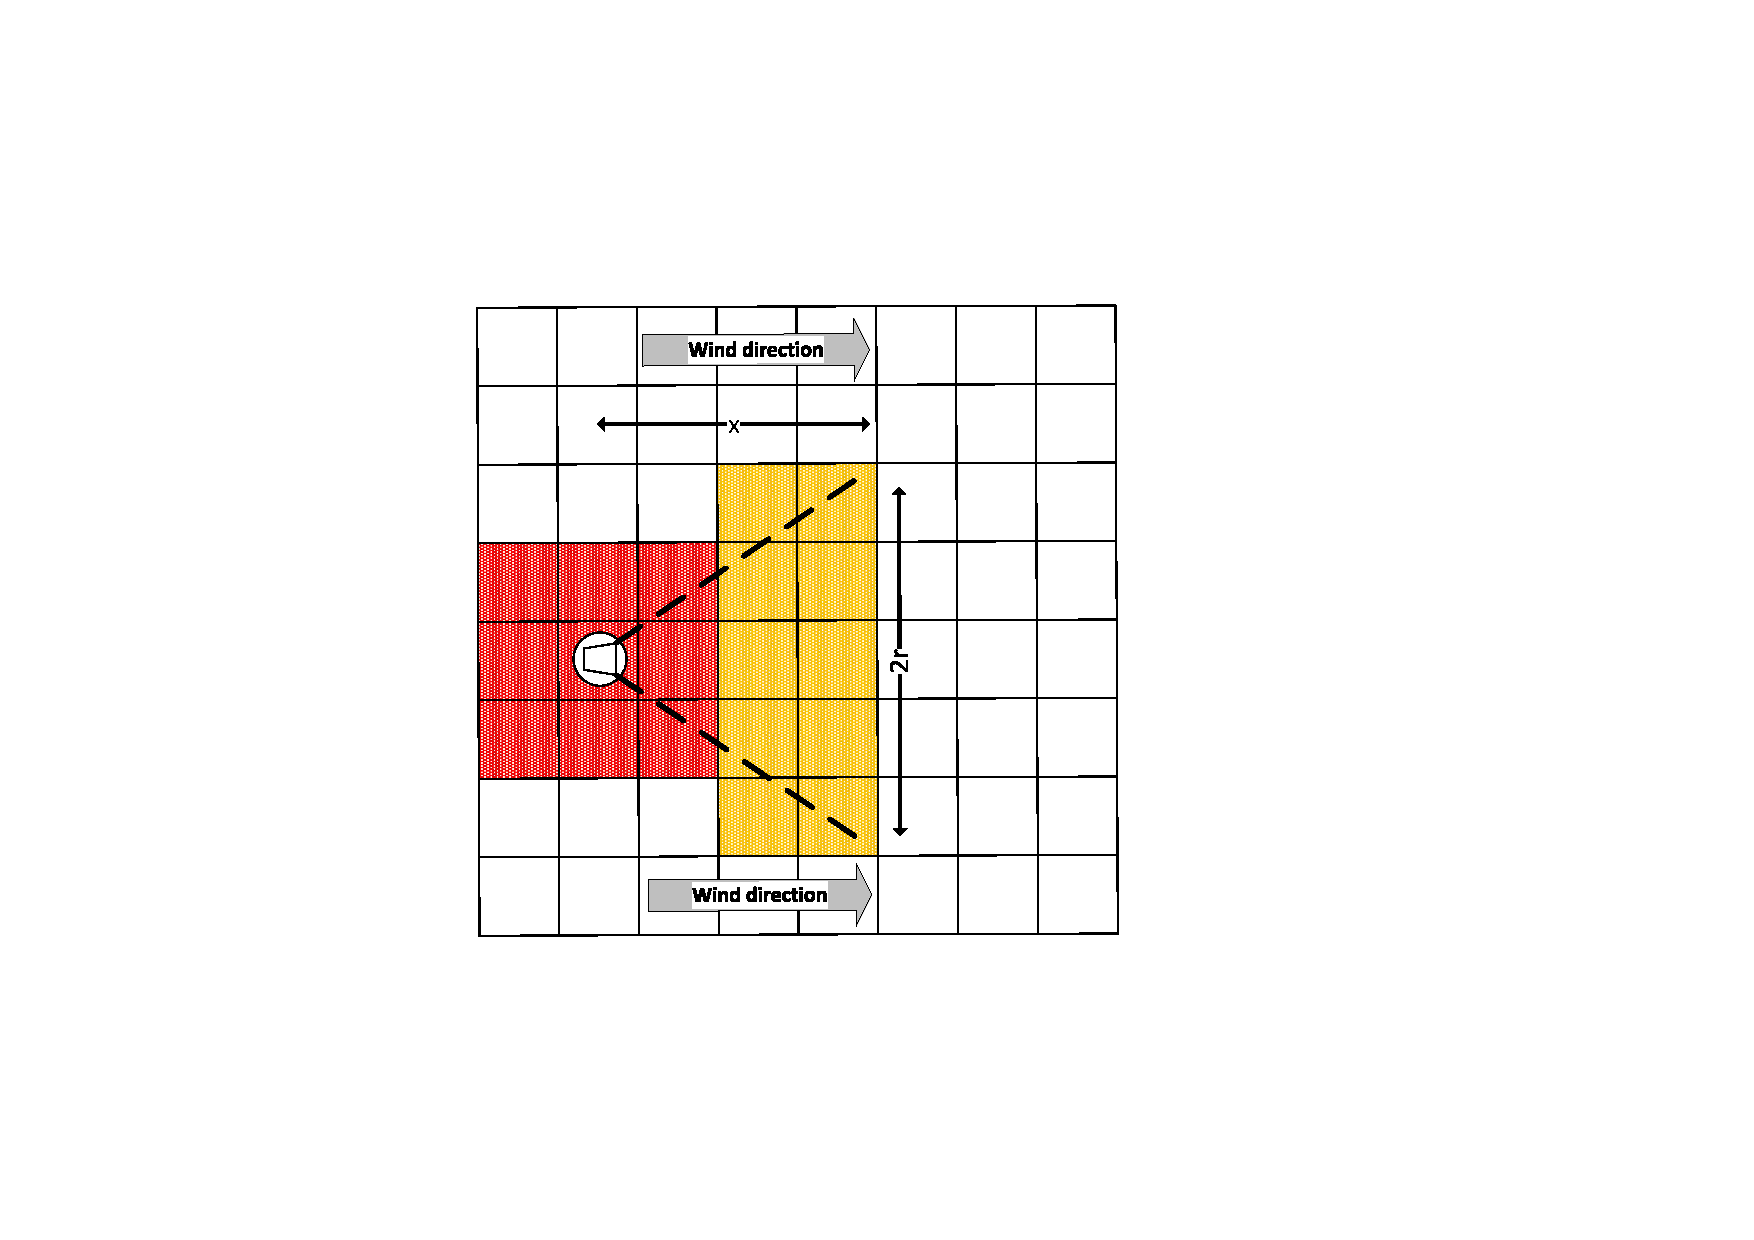
\includegraphics[scale = 0.9]{field_model.pdf}

	\caption{Wind farm model: proximity constraints, wakes, wind direction.}\label{fig:field_model}
\end{figure}



\paragraph{Proximity Constraints}
Turbines must be placed at least \emph{five rotor diameters}
apart. Depending on the cell size, we formulate the
corresponding constraint as part of the optimization model. For
example, if a turbine is placed in the center of a
cell, a cell size of $c = 100$ meters and a rotor diameter
of $40$ meters, requires that two turbines are not placed in adjacent cells. In Figure~\ref{fig:field_model}, the red area
around the turbine represents the forbidden cells. Conversely, if $c = 200$ and turbines are placed in the center of the cell, no proximity constraints are required as the required separation is enforced by the granularity of the spatial discretization.
	 
\paragraph{Wakes}
Turbines influence each other through \emph{wake} interference effects that reduce the effective power produced by a turbine due to upstream turbines that change the airflow dynamics~\cite{jensen1983note,shakoor2016wake}.
%that are
%referred to as \emph{wakes}~\cite{jensen1983note,shakoor2016wake}.
 In
Figure~\ref{fig:field_model}, the wind is assumed to be
blowing from left to right. The wake effect due to placing the turbine
expands as shown in the diagram.
%: it will influence only turbines that
%are placed in the orange cells.  In other words,
If a turbine is placed in the orange area, its effective power is
reduced due to the upstream turbine.
% that we placed in the $8\times8$ farm.
Moreover, a given turbine may be placed downstream from multiple turbines and hence
multiple wakes must be taken into account for each location.  The
reduction of power due to the wake effect is determined by three
parameters: (1) the distance between the upstream turbine and the cell
for which we want to compute the effect (denoted by $x$ in
Figure~\ref{fig:field_model}), (2) the radius of the cone's opening at distance $x$ 
(denoted by $r$ in Figure~\ref{fig:field_model}), and (3) the
combination of several wind regimes where a wind regime consists of 
the wind's free speed and direction.  The wake effect can be pre-computed
for each pair of cells since we know the distance ($x$), the turbine
specifications and terrain conditions (that jointly dictate $r$), and the
probabilistic behavior of wind regimes~\cite{Zhang2014}.
	 
\paragraph{Effective Power Calculations in the Presence of Wakes} 
Let $\mathcal{D}$ be the set of wind regimes.
%where every regime, $d\in \mathcal{D}$, is a combination of wind direction and free speed. 
The probability of wind regime 
$d \in \mathcal{D}$ is given by $p_d$ with $\sum_{d \in \mathcal{D}}^{} p_d = 1$. In the experimental section (Section~\ref{sec:eval}),
we provide one example of a probability distribution 
function over $36$ wind regimes (Figure~\ref{fig:prob_wind}). In that example, 
one regime $d=(10^\circ, 12 \mbox{ km/h})$ corresponds to a north-easterly wind blowing at a free velocity of $12\mbox{ km/h}$. The
probability of this regime is $0.008$.

Let $u_{id}$ be the wind velocity at turbine $i = 1,\ldots, m$ for wind regime $d\in\mathcal{D}$.
%\footnote{Turbines can adjust their orientation according to the current wind regime.}
  Given the interference of the wakes, the velocity of turbine $i$ is not equivalent to the free wind speed of $d$.
Rather, $u_{id}$ can be computed using the following equation~\cite{Zhang2014}:
\begin{equation}
u_{id} = u_{id\infty} \Bigg[1 - \sqrt{\sum_{j\in\mathcal{U}_{id}} \bigg( 1-\frac{u_{ijd}}{u_{id\infty}} \bigg)^2}  \Bigg], \label{eq:ss}
\end{equation} with $u_{id\infty}$ being the free wind speed (the second component of regime $d$), $\mathcal{U}_{id}$ corresponding to the set of turbines  that are upstream to $i$ 
under wind regime $d$, and $u_{ijd}$ being the wake-reduced speed at $i$ due to upstream turbine $j$. 
The reduced speed, $u_{ijd}$, is computed using the distance $x$ between the two turbines ($i,j$)  and turbine and terrain specifications that yield the cone opening radius, $r$. The set of upstream turbines, $\mathcal{U}_{id}$ is computed  
by rotating the grid wrt to the current wind regime $d \in \mathcal{D}$ and identifying the turbines, $j$, located upstream of turbine $i$ given $d$. The expression in Eq. (\ref{eq:ss}) is referred to as the \emph{sum-of-squares} (SS) model for 
the total expected power in presence of wakes~\cite{Zhang2014}.  We can now write 
the sum-of-squares (SS) expected power of a wind farm with $m$ turbines:
%~(\cite{Zhang2014}):
\begin{equation}
  E_{SS} = \sum_{i=1}^m \sum_{d\in\mathcal{D}} \frac{1}{3} u_{id}^3p_d.\label{eq:ess}
\end{equation}

  Eq. (\ref{eq:ess}) is considered the most accurate analytical total power expression that accounts for multiple wakes~\cite{jensen1983note}. 
  However, the expression is challenging for exact mathematical optimization techniques due to its complexity (i.e., the cube of a square root).
  %since it is a squared root function of a cubic expression. 
  %Hence, a simplified representation for the total expected energy that considers wakes is required. 

An alternative 
form of the total expected power in the presence of multiple wakes is the linear superposition (LS) expression:

\begin{equation} \label{eq:ls}
E_{LS} = \sum_{i=1}^m \sum_{d\in\mathcal{D}} \Bigg(\frac{1}{3}u_{id\infty}^3 -\sum_{j\in\mathcal{U}_{id}} \frac{1}{3}(u_{id\infty}^3 - u_{ijd}^3)\Bigg).
\end{equation}

Note that $E_{LS}$ has the same parameters as $E_{SS}$ but differs in their relationship.
The LS model is less accurate compared to SS~\cite{Zhang2014}, yet as we will show in Section~\ref{sec:QUBO4WFLO}, it 
 results in a quadratic objective function in our WFLO formulations. Such functions have been the subject of recent research advances~\cite{ku2017hybrid,bian2010ising}, motivating the contributions here.
%, which is a desired property from an optimization standpoint. \todo{[JCB: A bit strange to claim that a quadratic model is ``natural'' in the abstract but then argue that the model we adopt is an approximation but it is good because it is quadratic. Sounds like it is not natural and we choose it due to its optimization properties. Arik: I changed the arguments - please see the abstract and the beginning of the introduction.]}
 

\subsection{Optimization Methods for WFLO}

The allocation of turbines in a grid-like wind farm was first
considered as an optimization problem by~\citet{MOSETTI1994105}. Their
method employs a genetic
algorithm~\cite{davis1991handbook}, an approximate technique
with no guarantees of solution quality but with the goal of quickly finding a high-quality turbine placement.

In subsequent work~\cite{turner2014new,Zhang2014}, 
the WFLO problem was solved using \emph{exact}  
optimization methodologies that guarantee that the returned solution is optimal with respect
to the specified objective or is provably within a given bound of optimal.
%(i.e., maximize total expected power). 
The exact methods were shown to yield higher energy values, yet they often suffered from 
high computational cost and long run-times. In practice, it is often desirable to strike a balance between optimality and computational requirements: fast sub-optimal solutions are useful when solving the wind farm design problem numerous times (e.g., when considering different numbers of turbines and various allowed locations), while optimal solutions yield the best possible placements (admitted by the mathematical model) when longer run-times are available.

In what follows, we provide a literature review that covers both exact and approximate methods for WFLO. We subsequently relate our 
work to both approaches via our proposed quadratic optimization framework for WFLO.\footnote{We review 
only literature that considers the same wind farm model as the one presented at the beginning of this section. For a broader literature review see Zhang et al.\ \cite{Zhang2014}.} 
 
\paragraph{Exact Optimization Methods} 
The WFLO problem can be solved  
to optimality, using
techniques from operations research (e.g., mixed-integer linear programming (MILP), quadratic programming (QP), and constraint programming (CP))~\cite{Zhang2014,turner2014new,donovan2005wind}.
These methods are \emph{exact}, in the sense that they guarantee that the returned solution is indeed
the best solution one can obtain for the given model of the problem. Donovan was the first to solve WFLO using a
MILP approach based on the LS energy expression~\cite{donovan2005wind}. Turner et al.\ \cite{turner2014new} approximated the SS energy expression using a quadratic and a linear approximation. The two resulting methods performed well when
compared to existing approximate and exact techniques.
Another non-linear optimization approach \cite{ulku2019new} relaxed the binary placement variables to continuous values in $[0,1]$
and approximated the constraints such that the resulting variables yield an integer placement.
Their approach provides another approximation to the WFLO problem considered by Turner et al.\ \cite{turner2014new}.

Zhang et al.\ \cite{Zhang2014} developed a constraint programming (CP) approach to the problem variation presented above. CP is an optimization technique that has grown from the AI literature that does not make the assumptions on the functional form of the constraints or objective \cite{rossi2006handbook}. The authors compared existing MILP and QP models to their approach for directly optimizing the SS objective and showed that, while promising for smaller problems, applying CP turned out to be computationally intractable for the larger standard WFLO benchmarks. 

%% The most recent attempt to solve the wind farm variation that we presented 
%% in this section is given in Zhang et al.\ \cite{Zhang2014}. The authors compared
%% previously existing MILP and QP models to their approach for directly optimizing the SS objective. To this end, they used constraint programming (CP), which 
%% is an optimization technique that does not make assumptions on the functional form of the objective.
%% However, applying CP turned out to be computationally intractable for the larger standard WFLO benchmarks. 

In our work, we build upon the approach in Donovan~\cite{donovan2005wind}, yet instead of using a linear version of the LS objective, we 
model WFLO using a quadratic representation. %The difference between our approach and the quadratic model
%proposed in
Unlike Turner et al.\ \cite{turner2014new} and Ulku and Alabas-Uslu\ \cite{ulku2019new}, our model is not an approximation of the SS objective, 
but rather an exact representation of the LS objective. That is, while the previous work has approximated a more accurate physical model, we are exactly representing the less accurate physical model: the approximation arises at a different stage of the modeling pipeline.

While the main advantage of exact techniques
is that they provide guarantees on solution quality, they may take a very long time to  find an optimal solution. 
In fact, Section~\ref{sec:QUBO4WFLO} shows formally that WFLO is computationally hard, a result
that is not surprising but that has apparently not explicitly appeared in the WFLO literature. Therefore,
when one considers solving multiple wind farm design problems, if a fast solution is of essence,
one may turn to approximate optimization techniques.

\paragraph{Approximate Methods} In contrast to exact methods, approximation algorithms often provide   
quick and, hopefully, sufficiently high-quality solutions. Several works have solved 
WFLO using evolutionary (genetic) approaches~\cite{MOSETTI1994105,gonzalez2010optimization,grady2005placement}. 
%These methods use two principles (cross-over and mutation)
%to change existing solutions and improve them over time.
These methods do not guarantee termination 
(i.e., they may run forever without achieving a quality criteria), and even when they do terminate they do
not guarantee optimal solutions. Hence, one must often
introduce non-quality related stopping criteria, 
compromising the quality of the obtained solution~\cite{davis1991handbook}.
Furthermore, it is awkward to introduce constraints into genetic methods (see e.g., \cite{sorkhabi2018constrained}), leading to potentially costly feasibility checks and problem-specific repair operations for every solution found. 

The first attempt to address these limitations 
was made using a local search approach~\cite{ozturk2004heuristic}. 
The approach does not guarantee optimality, 
yet it circumvents the termination and feasibility checking issues of the evolutionary
methods. The local search attempts to apply either move, remove or add actions given an incumbent 
feasible solution. When a turbine is moved, removed or added, the new solution is evaluated. The procedure terminates 
when a stopping criteria is reached.
The main limitation of this approach 
%~\cite{ozturk2004heuristic}
is that it cannot perform an action 
that leads to an infeasible state and, therefore, often quickly converges to a sub-optimal solution (local optimum) 
that can potentially be much lower quality than the globally optimal solution~\cite{rivas2009solving}. 

To overcome this limitation, Rivas et al.\ \cite{rivas2009solving} used simulated annealing (SA), 
a neighborhood search method that allows visits to infeasible solutions. 
SA creates a well-connected solution space that allows the algorithm to escape 
local optima. The SA method was shown to be superior to the approach of Ozturk \& Norman~\cite{ozturk2004heuristic} 
and to the genetic method proposed in Grady et al.\ \cite{grady2005placement}. A drawback of the SA approach 
is its ad-hoc nature. The various components of the algorithm
 must be tailored to the problem at hand and, as a result, small adjustments of the WFLO setting
 (e.g., adding noise considerations), would require major changes to the SA implementation. 
Additional methods and experimental comparisons between various approximate algorithms are available in Samorani~\cite{samorani2013wind}.

In our work, we also use an annealing based approach (similar to Rivas et al.\ \cite{rivas2009solving}). However,
our methodology is generic since it is based on a declarative problem model and
on the ability of specialized hardware to solve %(non-ad-hoc)
quadratic problems.


Recently, several efficient WFLO solutions based on developmental models were introduced~\cite{wilson2013learning,wilson2014continuous}. These works do not represent the actual underlying physical model of the system, and while providing fast solutions to WFLO,
they do not attempt to optimize on the actual objective function (that is, the total energy that a farm produced) nor capture the complexities of the underlying problem. For example, one approach~\cite{wilson2013learning} models turbine interference using a parametric probabilistic model (assuming a Weibull distribution). In our quadratic models, we explicitly represent the energy term, and the physical dependencies between the turbines (i.e., wakes and proximity constraints). Furthermore, our models
optimize an empirically established energy objective, the linear superposition expression in Eq.~(\ref{eq:ls}).

%\paragraph{Quadratic Programming as a Unified Framework for Exact and Approximate WFLO}
%\todo{send a clear message here. Perhaps move to next section}.



%
%
%Specifically, we consider two variations of the quadratic programming paradigm.  
%The first one is referred to as quadratic constrained optimization problems (QCOP). 
%It enables maximizing a quadratic (LS-based) energy expression, while 
%ensuring that WFLO constraints are maintained (turbine proximity and total number of turbines is $m$). 
%The second model is a quadratic unconstrained binary optimization (QUBO), 
%which 
%
%
%On the one hand, exact solvers for quadratic programs (QCOP and QUBO) such as Gurobi~\cite{}, 
%use cutting edge
%operations research methods to enhance performance.
%On the other hand, simulated annealing methods have been recently embedded onto 
%designated processing units. These units use quantum-inspired technology to solve
%complex problems quickly and with minimal degradation in terms of the resulting solution~\cite{}.
%Specifically, in this work, we shall use Fujitsu's digital annealer (DA) to solve WFLO. The DA
%also requires a quadratic representation of the WFLO problem. 
%
%Both of these methods use 
%quadratic optimization models, which we shall present in the next section (Section~\ref{sec:QUBO4WFLO}).
%


\section{Quadratic Models for WFLO}
\label{sec:QUBO4WFLO}

A benchmark study comparing state-of-the-art exact approaches \cite{Zhang2014} to 
approximate methods found that the two perform in a comparable fashion, without large differences between
the attained energy~\cite{yang2019simulated}. Exact methods tend to perform slightly better
in smaller WFLO benchmarks, while simulated annealing methods dominated for larger standard WFLO benchmarks. 
These results led to the conclusion that both types of methods (exact and approximate) should be considered. Therefore, we introduce a unified paradigm, namely quadratic programming, that enables
both exact and approximate solutions to WFLO. Further, formulating WFLO using quadratic programming enables us to employ 
recent advanced exact software solutions (e.g., Gurobi optimizer) and approximate hardware developments 
(e.g., Fujitsu's Digital Annealer).
%Thus, 
%our approach `enjoys' the best of both worlds (the exact and the approximate). 

%In this work, we argue that 

%that solves quadratic problems using principles from simulated annealing). 

%% In this section,
%% we formulate the WFLO problem
%% using quadratic programming. Specifically,
We consider two
quadratic optimization problems that represent WFLO: a
quadratic constrained optimization problem (QCOP) and 
a quadratic unconstrained binary optimization (QUBO) problem. 
The former represents WFLO characteristics (proximity and number of turbines)
as hard constraints, while the latter considers these characteristics as soft constraints such that the objective function is penalized in case these
constraints are violated.

We start by presenting the inputs and decision variables of our optimization approaches.
Subsequently, we introduce the two quadratic formulations of WFLO and 
prove its computational complexity. Lastly, we discuss the details of existing
software and hardware solutions that can be used to solve the two formulations. 

\subsection{WFLO Inputs and Decision Variables}
Given the wind farm problem presented in Section~\ref{sec:related},
let $x_i$ be a binary decision variable that represents whether a 
turbine is positioned at location 
$i \in \mathcal{N}$ with $\mathcal{N}$ being the set 
of $k = n^2$ possible turbine locations (cells in the grid). We 
write $x$ as shorthand for $x = (x_1,\ldots, x_k)$. 
We denote by $\mathcal{E} \subseteq \mathcal{N}\times \mathcal{N}$
the set of location pairs that cannot simultaneously host turbines 
due to proximity constraints. The set $\mathcal{E}$ can be pre-computed 
based on problem specifications.
%For example,
%it is common to assume that two turbines must be placed at least five rotor diameters apart. 

Let $u_{id}$ and $u_{id\infty}$ 
be the wind speeds at turbine location $i \in \mathcal{N}$ for wind regime $d \in \mathcal{D}$
with and without interference from other turbines due to wake effects, respectively. 
Note that here we refer to $i$ as a potential turbine location and not the $i$th turbine as we did in Section~\ref{sec:related}.
Further, we denote by $\mathcal{U}_{id} \subseteq \mathcal{N}$ 
the set of upstream 
turbine locations for wind regime $d$
given that a turbine is placed at cell $i$ (i.e., turbines placed in these locations 
will influence a turbine placed in $i$). Finally,
we denote by $u_{ijd}$ the wind speed at location $j$ due to a single wake from upstream turbine at location $i$ with $j \in \mathcal{U}_{id}$. 
The following function  
represents the total expected energy of a wind farm given placement decisions 
$x$: \begin{equation}
f(x) = \sum_{i \in \mathcal{N}}^{} \sum_{d \in \mathcal{D}}^{} p_d ( \frac{1}{3} \ u_{id, \infty}^3 x_i  - \sum_{j \in \mathcal{U}_{id}}^{} \frac{1}{3}(u_{id, \infty} ^3 - u_{ijd}^3)x_i x_j).   \label{ObjFunc}\\
%&s.t.:& \nonumber\\
%&\mbox{       }& \sum_{i \in \mathcal{N}}^{} x_i = m,\label{Cardinality}\\
%&\mbox{       }& x_i + x_j \leq 1,   \forall (i,j) \in \mathcal{E}, \label{Grid}\\
%&\mbox{       }& x_i \in \{0,1\},     \forall i \in \mathcal{N}.
\end{equation} The objective function corresponds to the linear superposition (LS)
expression (c.f., Eq.~\ref{eq:ls} in Section~\ref{sec:related}). We are now ready to provide the two quadratic programs to represent WFLO.

\subsection{WFLO as a Quadratic Constrained Optimization Problem}

To 
maximize $f(x)$ and satisfy the total number of turbines and proximity 
constraints we write
the following quadratic constrained optimization problem (QCOP):
\begin{eqnarray} \label{QCOP}
&\max_{x_i}^{}& \sum_{i \in \mathcal{N}}^{} \sum_{d \in \mathcal{D}}^{} p_d ( \frac{1}{3} \ u_{id, \infty}^3 x_i  - \sum_{j \in \mathcal{U}_{id}}^{} \frac{1}{3}(u_{id, \infty} ^3 - u_{ijd}^3)x_i x_j)   \\
&s.t.:& \nonumber\\
&\mbox{       }& \sum_{i \in \mathcal{N}}^{} x_i = m,\label{Cardinality}\\
&\mbox{       }& x_i + x_j \leq 1,   \forall (i,j) \in \mathcal{E}, \label{Grid}\\
&\mbox{       }& x_i \in \{0,1\},     \forall i \in \mathcal{N}. \label{Vars}
\end{eqnarray} Constraints~\ref{Cardinality}~and~\ref{Grid} ensure that exactly $m$ turbines are placed on the grid
and enforce proximity constraints between the turbines, respectively. We shall refer to the QCOP
formulation of WFLO as \qcls{}. 

\qcls{} can be solved using an exact optimization solver, e.g., Gurobi~\cite{gurobi}. 
Linear versions of the QCOP (\qcls) have been previously proposed and solved using the corresponding exact solvers~\cite{Zhang2014,donovan2005wind}.
%\todo{JCB: We need to formally present the ILP model in the experiment section. We can then discuss the fact that the model is identical - because the linearization gives and exact representation. Should put a forward reference to that model here.}
%\todo{Are these linear formulations ``equivalent'' as you claimed or approximations? If they are mathematically equivalent, why do we think a quadratic model will be any better computationally? Arik: The two formulations are equivalent to WFL-QCOP. However, we compare against the ILP model experimentally and it does worse than WFL-QCOP. Hopefully, Jason's part in Section 3.5.1. based on Wen-Yang's thesis will explain why it does better. Originally, I used the quadratic formulation because it seemed more natural. Semantically, the linear model and the quadratic model are the equivalent imho.}



\subsection{WFLO as a Quadratic Unconstrained Binary Optimization Problem}

Quadratic unconstrained binary optimization problems (QUBOs), as their name implies, do not allow the direct representation of hard constraints. Instead, 
%they only 
%have an objective function that 
%one can to maximize (or minimize) and
problem constraints must be represented as part of the objective function
using penalty terms. 

Let $\lambda = (\lambda_1,\lambda_2)$ 
be a vector of constraint weights with $\lambda_i >0$. The equivalent QUBO formulation of the QCOP in Eq. (\ref{QCOP}) is given by,
\begin{equation}\max_{x}^{} f(x) - \lambda_1 (\sum_{i \in \mathcal{N}}^{} x_i -m) ^2 - \lambda_2 \sum_{(i,j) \in \mathcal{E}}^{} x_i x_j , \label{QUBO}\end{equation}
with the term $ \lambda_1 (\sum_{i \in \mathcal{N}}^{} x_i -m) ^2$ 
penalizing solutions that violate the exactly $m$ turbines constraint and the term $\lambda_2 \sum_{(i,j) \in \mathcal{E}}^{} x_i x_j$ penalizing
solutions that violate the proximity constraints. The two penalty terms $\lambda_1$ and $\lambda_2$ 
must be large enough to ensure that the solutions are indeed feasible wrt the problem constraints. We shall refer to the QUBO representation of WFLO as \quls.
%These types of constraints
%are referred to as \emph{soft constraints} as they do not guarantee a feasible solution 
%for an arbitrary selection of $\lambda$.   

\subsection{The Computational Complexity of \qcls{}}
\label{sec:computational}
%(linear) problems were formulated and solved using  exact solvers.
Despite the existence of mathematical models for WFLO in the literature~\cite{Zhang2014,donovan2005wind} that are expressive enough to represent $\mathcal{NP}$-hard problems, we are unaware of an explicit treatment of the computational complexity of WFLO.
%However, these solvers should only be used if the problem is computationally hard.
%We are unaware of an existing complexity result for the LS variation of WFLO (our QCOP).
We therefore provide a straightforward proof of the computational complexity of \qcls{}. 

\begin{mythm}
	The computational complexity of \qcls{} defined in \eqref{QCOP}-\eqref{Vars} is $\mathcal{NP}$-hard. 
\end{mythm}
\begin{myproof}
We prove by showing that a special case of the \qcls{} \eqref{QCOP}-\eqref{Vars}  is
$\mathcal{NP}$-hard. Suppose that $\mathcal{E} = \emptyset$, i.e., the grid is coarse-grained enough to ignore proximity constraints. Then, the constraints in Eq.~(\ref{Grid})
are dropped and we get the heaviest k-subgraph problem, which is a known $\mathcal{NP}$-hard problem~\cite{billionnet2005different}.
Since a special case of \qcls{} is  $\mathcal{NP}$-hard,  \qcls{} is at least $\mathcal{NP}$-hard. On the other hand,
\qcls{} is formulated using integer programming (Problem \ref{QCOP}), which means that it is at most $\mathcal{NP}$-hard. Therefore, we get that \qcls{} is $\mathcal{NP}$-hard.
\end{myproof}

%\todo{The proof is a bit awkward as it goes back-and-forth between QCOP and WFLO. Technically, the problem as defined in \eqref{QCOP}-\eqref{Vars} but, given the different (not mathematically equivalent) models of WFLO, this is different from claiming that WFLO is NPC. On the other hand, we so not want to prove that QCOP in general is NPC. So we need to get the language precise. Arik: I fixed it by referring to the problem as WFL-QCOP (and WFL-QUBO for the other one.)}

%To overcome the challenge associated with the computational hardness of WFLO,
%we reformulate the QCOP into a QUBO problem, which allows us to solve WFLO using specialized optimization hardware.  

\subsection{Solving QCOP and QUBO using Advanced Optimization Methods}

\subsubsection{QCOP solving methods}
\label{quadratic}
\qcls{} is a strictly convex integer 
quadratically constrained optimization problem (IQCOP), which is notorious for its computational complexity~\cite{van1981another}.
%In fact, we proved in Section~\ref{sec:computational} that WFL-QCOP is $\mathcal{NP}$-hard.
The common exact methods for solving
IQCOPs are tree search \cite{land2010automatic} algorithms with a variety of sophisticated techniques to limit the search necessary to find and prove optimality.  In operations research, the generic exact approach for solving IQCOPs is the branch-and-cut based mixed integer programming (MIP) \cite{bonami2008algorithmic}.

%A MIP solver, such as the one we use (Gurobi), uses a linear or quadratic continuous relaxation to efficiently compute a bound on the objective function. This relaxation is used to generate cuts, implied constraints that tighten the relaxation, to identify sub-trees that can be discarded without search because they are guaranteed not to contain a solution better than the current incumbent, and to drive the heuristic branching that systematically searches for a solution. %Typically, this process of cut generation, reasoning about sub-trees, and branching is performed at each node in the search tree.

Commercial MIP solvers have seen extensive development over the past 20 years with hardware-independent algorithmic improvements have delivered orders of magnitude improved performance \cite{Bixby07a}. More recently the development of such solvers has focused on representing and solving quadratic problems such as \qcls{}~\cite{Furini19a}.
%By solving a relaxed problem to bound the objective value at each node and strengthening the relaxed problem with cutting planes to restrict the feasible region further, MIP solvers has been proved effective for attacking IQCOPs \cite{junger200950}.

%Constraint programming (CP) \cite{rossi2006handbook} is another tree search framework that can be applied to solve IQCOPs. At each node in the search tree, inference algorithms that are often encapsulated in the global constraints \cite{katriel20066}, conduct domain filtering on each constraint. Domain filtering removes possible values from variable domains by proving that a value cannot satisfy the constraint and hence cannot appear in a global solution, hence pruning sub-trees with variable assignments that are not part of any feasible solution.

%In the community of communications, IQCOPs are commonly solved via discrete ellipsoid-based search (DEBS), which is built on enumeration of integer points in the hyper-ellipsoid defining the feasible region \cite{agrell2002closest}. DEBS can be interpreted as a form of CP, where the ellipsoid geometry induces for each variable an interval domain, producing an inference algorithm removing values that do not belong to the ellipsoid. However, DEBS cannot be applied to general IQCOPs due to its special nature. This drawback has been partially overcome by Wen-Yang \cite{ku2017hybrid}, who has proposed a competitive hybrid algorithm that combines DEBS and MIP to solve IQCOPs.

% In addition to exact methods, heuristics that are designed to find good but not provably optimal solutions fast can also be used to solve IQCOPs. 



%\todo{@Chris and Jason: I still feel that we need to say how Gurobi do it (or at least how we think Gurobi does that)}

\subsubsection{Specialized Hardware for QUBO}

Recent years have seen significant advancement in the use of specialized hardware platforms, such as adiabatic and gate-based quantum computers, Digital/CMOS annealers, and neuromorphic computers \cite{coffrin2019evaluating}, to solve hard combinatorial optimization problems. A large number of these platforms support the optimization of quadratic functions over binary variables by using Ising models \cite{johnson2011quantum}, an equivalent representation to QUBO \cite{bian2010ising}, as their mathematical abstraction.

In this work, we use the first generation of the Fujitsu Digital Annealer (DA) \cite{aramon2019physics}, a specialized CMOS hardware capable of solving QUBO problems with up to 1024 binary variables. The algorithm used by the DA is based on simulated annealing \cite{kirkpatrick1983optimization}, however it takes advantage of the massive parallelization provided by the custom CMOS hardware and uses a dynamic offset mechanism to escape local minima \cite{aramon2019physics}. The Fujitsu Digital Annealer has been previously applied to variety of problems in different research areas such as machine learning \cite{cohen2020ising,salehinejad2019ising} and communication \cite{naghsh2019digitally,rahman2019ising}.

Unlike %exact techninques
standard exact optimization solvers that run until obtaining an optimal solution, the DA runs until reaching a time limit and returns the best found solution.  In our experiments, we analyze the quality of obtained solutions for different time limits.


\section{Evaluation}
\label{sec:eval}

In this section, we 
present an numerical evaluation of the two quadratic models based on 
12 standard WFLO instances.
Our main results are: \begin{itemize}
	\item For given time limit, the Digital Annealer (DA) achieves a solution quality as good or as better than existing state-of-the-art exact methods on 10 of 12 instances.
		\item To achieve such a solution quality, the runtime for solving \quls{} on the DA is at least two orders of magnitude shorter than \qcls{} on state-of-the-art commercial solvers for hard WFLO instances.  
	\item Given sufficient runtime, solving the \qcls{} model with commercial software yields strong results on most of the instances. Compared to previous exact models (such as \qcss), \qcls{} is able to find equal or better solutions on 8 of 12 benchmark problems and for 5 of the 6 hard ones. %  \todo{Arik: Is this correct? Table 2 shows DA@10seconds with the best solution found for 7/12 instances and \qcls{}grb@3600 for 6/12. And 4/6 vs. 3/6 for the WR36). Are you comparing \qcls{}grb with \qcssgrb and ILP-LS? We seem to be underplaying DA performance in this comment. Chris: I changed to competitive results. You're right, I'd say that the DA is not `losing' to \qcls{}grb.}  
\end{itemize}

We start by outlining the experimental design of our evaluation, followed by an overview of our main results,
and conclude the section with a discussion of the results and their practical implications.

\subsection{Experimental Design}



\paragraph{Standard WFLO Instances}

To test and benchmark our models, we used 12 standard benchmark WFLO instances
from the literature~\cite{MOSETTI1994105,Zhang2014,grady2005placement} that we denote with the set $\mathcal{W}$. 
The 12 benchmarks result from varying 2 wind settings (1 and 36 wind directions),
2 grid sizes ($10\times10$ with cell size $200$ meters and $20\times20$ with cell size $100$ meters),
and 3 variations for number of turbines ($m \in \{20, 30, 40\}$). 
For the $36$ wind directions setting, the velocities come from the probability distribution presented in Figure~\ref{fig:prob_wind}.
%We denote $\mathcal{W}$ the set of 12 instances.
Instances with $36$ wind regimes are considered computationally more challenging~\cite{Zhang2014}.

Additional parameters that were used to calculate 
the velocities ($u_{id\infty}, u_{ijd}$) include: turbine height ($60$ meters),
ground roughness ($0.3$ meters), turbine rotor radius ($20$ meters), and a wind farm of size $2 \mbox{km} \times 2 \mbox{km}$.\footnote{The implementation of constructing the 12 standard WFLO instances can be found in~\url{https://bit.ly/2YIjTl1}.}


\begin{figure}[t]
	\centering
	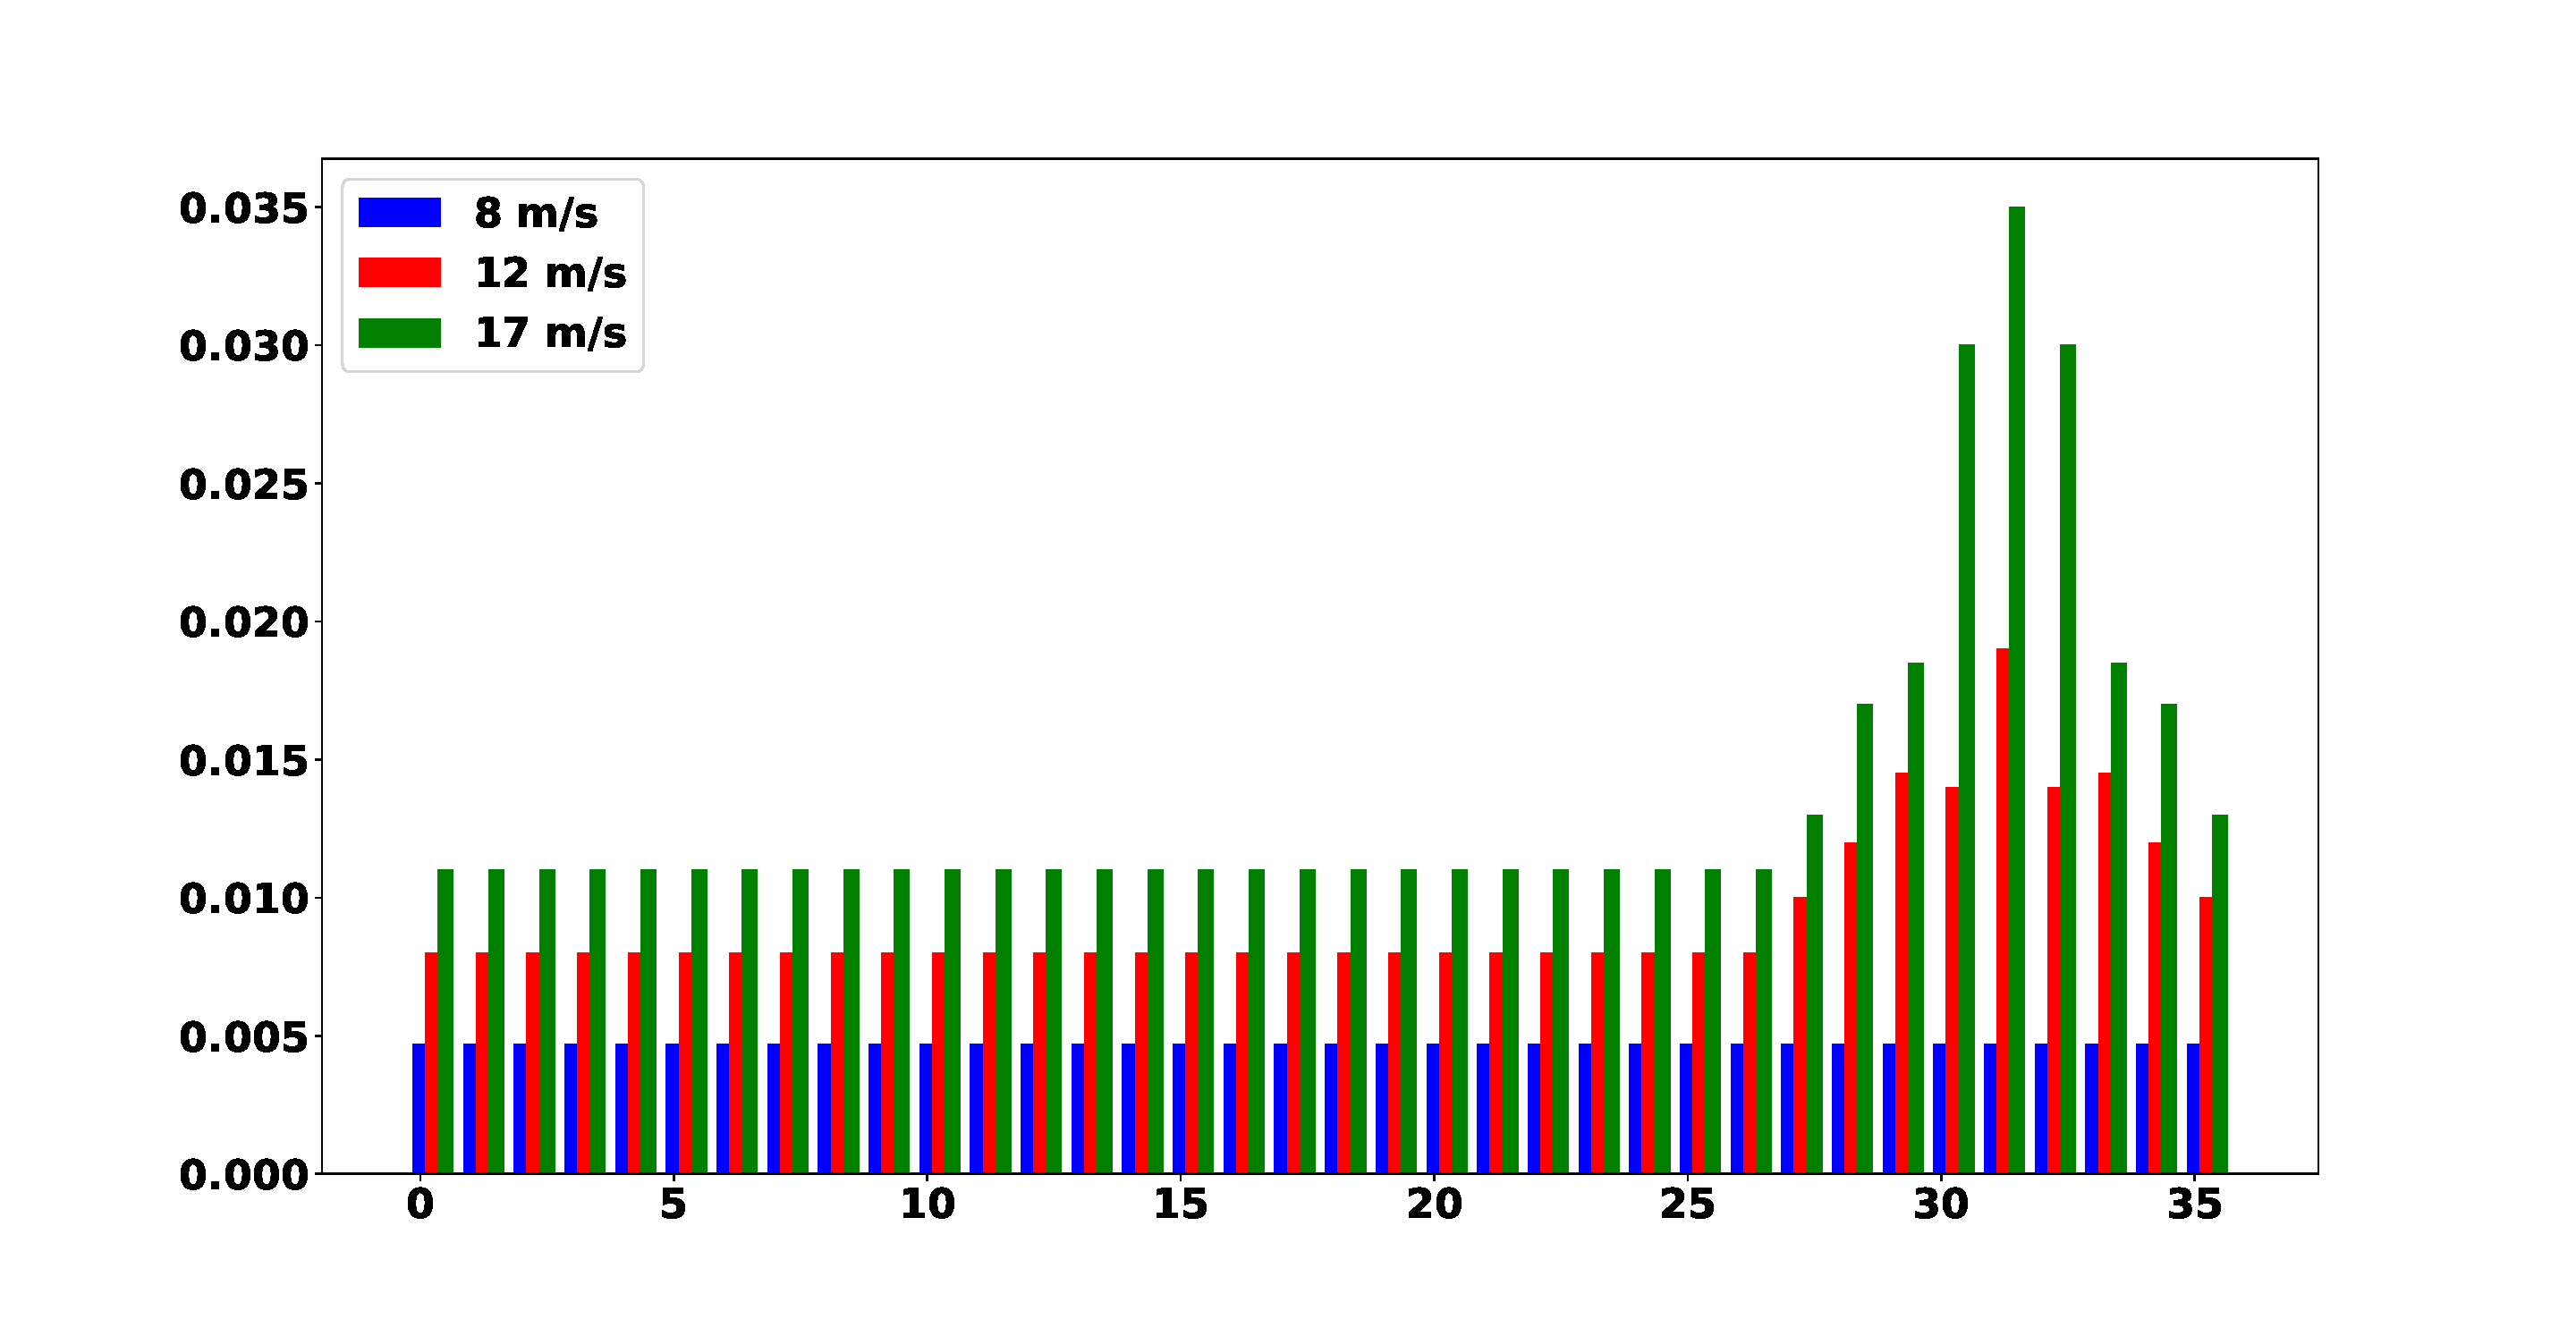
\includegraphics[scale = 0.3]{prob_wind_pdf.pdf}
	
	\caption{Wind regimes: x-axis is the angle (times 10 degrees), y-axis is the probability for wind regime, and color corresponds to free wind speed for the different wind directions.}\label{fig:prob_wind}
\end{figure}

\paragraph{Optimization Benchmarks}

We compared our two models, \qcls{} and \quls{}, against two state-of-the-art exact optimization methods:
the integer linear programming (denoted \ilpls) approach~\cite{donovan2005wind,Zhang2014} and the 
model that uses a quadratic approximation (\qcss)~\cite{turner2014new}. 
The ILP model is a standard, exact linearization of the \qcls{} model.
%% given in the following set of equations, which we denote WFL-ILP, \begin{eqnarray} \label{ILP}
%% &\max_{x_i}^{}& \sum_{i \in \mathcal{N}}^{} \sum_{d \in \mathcal{D}}^{} p_d ( \frac{1}{3} \ u_{id, \infty}^3 x_i  - \sum_{j \in \mathcal{U}_{id}}^{} \frac{1}{3}(u_{id, \infty} ^3 - u_{ijd}^3)y_{i,j})   \\
%% &s.t.:& \nonumber\\
%% &\mbox{       }& \sum_{i \in \mathcal{N}}^{} x_i = m,\label{Cardinality2}\\
%% &\mbox{       }& x_i + x_j \leq 1,   \forall (i,j) \in \mathcal{E}, \label{Grid2}\\
%% &\mbox{       }& x_i + x_j -1 \leq y_{i,j},  \forall i,j \in \mathcal{N}, \label{Linearization}\\
%% &\mbox{       }& y_{i,j} \geq 0,     \forall i,j \in \mathcal{N}, \label{Yij}\\ 
%% &\mbox{       }& x_i \in \{0,1\},     \forall i \in \mathcal{N}. \label{Vars2} 
%% \end{eqnarray} The variables $y_{i,j}$ are continuous and can take only non negative values (Eq.(\ref{Yij})). However, due to Eq.~(\ref{Yij}) their values must
%% be either zero or one. If a turbine is placed in both $i$ and $j$ ($x_i = x_j = 1$), then $y_{i,j}$ will be $1$ and a wake reduction 
%% will take place in the objective function. If a turbine is placed in either $x_i$ or $x_j$ (but not in both), $y_{i,j}$ will
%% take the value of $0$ and no wake reduction will occur. The WFL-ILP is equivalent to WFL-QCOP: the interaction
%% variables $y_{i,j}$ of the ILP model are replaced by multiplicative expressions $x_{i}x_{j}$, which makes Constraint (\ref{Yij}) redundant. 
However, the ILP is solved using linear optimization approaches, while \qcls{} is solved using quadratic programming methods as mentioned in Section~\ref{quadratic}. Hence
we can expect a difference in the performance of optimization software when solving the two problems. 


The existing constraint programming approach was
reported to perform worse than the ILP model~\cite{Zhang2014} and so was omitted from our the experiments.
We used state-of-the-art commercial software, Gurobi~\cite{gurobi}, to solve \qcls{}, \ilpls{} and \qcss. 
We shall denote the problems using their names and the solvers used as follows: \qclsgrb{} (GRB for Gurobi), \ilplsgrb{}, and \qcssgrb{}.
In addition, we 
used both Fujitsu's Digital Annealer and Gurobi to solve \quls: we shall refer to the former as \qulsda{} and to the latter
as \qulsgrb.


\paragraph{Experimental Procedure}

For exact methods (\qcss{}, \ilpls{}, \qcls{} and \quls{}),
we ran Gurobi with a time limit of 3600 seconds. We collected all feasible solutions
found until that point in time. The exact methods were solved using Gurobi's integer programming and quadratic programming solvers on a 
Ubuntu PC with Intel(R) Core(TM) i7-9700 8 core CPU@3.00 GHz with 12 MB cache and 8 GB RAM.

For the DA, we used a single configuration that was found to work best across the different instances. 
The DA was run for increasingly large time limits ranging from $0.7$ seconds to $65$ seconds where we no longer observe an improvement in 
performance. The penalty terms $\lambda_1$ and $\lambda_2$ (see~Eq.~\eqref{QUBO}) are selected such that $\lambda_1= \lambda_2$ and sum of the two penalty terms, namely $\lambda_1+\lambda_2$, 
is the highest value that the Digital Annealer allows.\footnote{The DA has an upper limit on the size of objective function coefficients.} 
 


%The best solution in terms of energy is the solution that attained the highest objective
%values (SS in \qcssgrb and LS in the rest of the methods).
 


%
%The initial temperature \text{tmp\_st} is 500000, the temperature mode is 0, the interval \text{tmp\_interval} for updating is 1, the offset increase rate is 10, the number of runs is 20, and the temperature decay rate is computed dynamically, i.e., $ \text{tmp\_decay} = (0.001 / \text{tmp\_st})^{(1.0 / (\text{num\_iterations} / \text{tmp\_interval}))} $. This formula of decay rate is for better convergence and is provided by DA developers. \todo{JCB: Yes, if it is not too complicated. You should mention if this is the standard thing that DA does or something you came up with.} The DA ran until convergence of the underlying simulated annealing algorithm and the runtime 
%of the procedure was recorded. \todo{\\EC: I am not sure what does it mean for the DA to run until convergence. You may want to specify that the DA was run with increasingly large time limits until no further improvement in objective.\\}
%
%
%\todo{@Chris: do we want to share the code that ran the experiments in batches? perhaps it should be separated from the problem construction and the two need to be shared separately.} \todo{JCB: As I requested last fall, we should have separate problem instance files from the code and make at least the problem instances available. Arik: OK, we will upload the experiment to the github and share the link.} 



\paragraph{Performance Measurement} 

We measured the total expected energy of a solution using the SS expression (see Eq.~(\ref{eq:ss})).
%\footnote{The total mean energy is presented in kW.}.
The only method that directly optimizes SS is \qcssgrb{}. Hence, for the other methods, we converted
LS-based solutions into the SS expression using Eq.~(\ref{eq:ss}) as proposed in Zhang et al.\ \cite{Zhang2014}. Specifically, let $x = (x_1, \ldots, x_k), k=n^2$ be a turbine placement solution obtained by an LS-based method.
Then, the SS energy expression can be written as, 
$$\sum_{i\in \mathcal{N}}\sum_{d \in \mathcal{D}} \frac{1}{3} x_i \Bigg(u_{id,\infty} \Bigg[1-\sqrt{\sum_{j\in \mathcal{U}_{id}}x_j\bigg( 1-\frac{u_{ijd}}{u_{id,\infty}} \bigg) } \Bigg]    \Bigg)^3.$$ 

Next, we tested the performance of our approach as function of solution time. We 
compared the average performance of all WFLO methods on all 12 WFLO instances. Since energy levels are not directly comparable between the different instances (due to varying number of turbines and wind farm specifications) we used the \emph{mean relative error} (MRE) measure with respect to the best solution obtained per instance.
%Then, the
%time-varying MRE can be averaged across the 12 scenarios and presented over time.
%In what follows, we demonstrate the construction of the MRE measure.

Recall that $\mathcal{W}$ is the set of our 12 standard WFLO instances. 
Let $b_w$ be the best energy solution (in terms of SS) obtained for an instance $w \in \mathcal{W}$ 
across the different methods.
%For example, the best solution (within 3600 seconds) for the second instance $w_2$ that aims at placing $30$ turbines on a $10\times10$ grid with a single wind regime is attained by \qulsgrb and the SS energy expression is $15742$ (kW); thus, we set $b_w = 15742$.
Then, for every point in time $t \in \{0,\ldots, 3600\}$ (measured in seconds), we can compute the relative error of a given approach per instance $w$. Let $\mathcal{A}$ be the set of solution approaches, $$\mathcal{A}= \mbox{
	\{\emph{\qulsgrb}}, \mbox{\emph{\qclsgrb}}, \mbox{\emph{\qulsda}}, \mbox{\emph{\ilplsgrb}}, \mbox{\emph{\qcssgrb}}\}.$$ Further, denote by $b_{w,t,a}$ the best solution attained before time $t$ by approach $a$ for instance $w$. Then, the relative error at time $t$ for approach $a$ on instance $w$ is given by
\begin{equation}
  RE(w,t,a) = \frac{b_w - b_{w,t,a}}{b_w}.
\end{equation} Note that the expression is always non-negative, since we are solving a maximization problem. We can now average over the different instances at time $t$. The average performance of approach $a$ at time $t$, $MRE(t,a)$ can be computed as, \begin{equation} MRE(t,a) = \frac{1}{|\mathcal{W}|}\sum_{ w\in\mathcal{W}} RE(w,t,a).\end{equation}
We present $MRE(t,a)$ for each of the approaches to demonstrate the speed of convergence of the proposed LS-based methods.

The last measure that we introduce is the speed-up factor $S(a_1, a_2, t, w)$. The measure compares the time that it takes
approach $a_1 \in \mathcal{A}$ to
achieve the same energy level as the energy achieved by approach $a_2 \in \mathcal{A}$
within $t$ seconds when solving instance $w$ (energy levels are measured in terms of the sum-of-squares energy expression). 
Formally, \begin{equation} S(a_1, a_2, t, w) = \frac{\min \big[\{ t' : E_{SS}(a_1, t',w) = E_{SS}(a_2, t, w) \} \cup \{3600\} \big] }{t}, \label{eq:speedup} \end{equation}
with $E_{SS}(a, t, w)$ being the SS energy value under approach $a$ for instance $w$ at time $t$. The speed-up factor 
is useful to measure how many times faster (or slower) approach $a_1$ solves problem $w$ compared to approach $a_2$.   
For example, $$S(\mbox{\emph{\qclsgrb}}, \mbox{\emph{\qulsda}}, 10, w_1)$$ is the ratio between the time that it takes \qclsgrb{} to 
reach the same quality of solution as \qulsda{} achieves after $10$ seconds on problem $w_1$. Since
we limit the runtime of the exact methods by $3600$ seconds, $S$ is a lower bound on the true speed-up factor. 
%Therefore, if for the example above the result is $3600/10$, we shall interpret it as a speed-up factor of \emph{at least} $360$. 


\subsection{Main Results}

%% In this part, we present the main findings of our empirical evaluation. 
%% We shall start by showing the best attained solutions by all methods.
Table~\ref{tab:results1} contains the best energy (in kW) attained by the methods
for the 12 WFLO instances after $100$ seconds of runtime for the exact methods. 
The runtime for the DA was always less than $10$ seconds.


\begin{table}[t!]
	\small
	\begin{tabular}{| c | c | c | c | c | c | c | c |}
		\toprule
		Wind Directions  & n  & m  & \qulsda{}  & \qulsgrb  & \qcls & \qcss  & \ilpls  \\
		\toprule
		\multirow{6}{*}{WR1}  & \multirow{3}{*}{10}       & 20       & \textbf{11185.41} & \textbf{11185.41} & \textbf{11185.41} & \textbf{11185.41} & \textbf{11185.41} \\
		& & 30   & 15740.69 & \textbf{15742.93}  & 15738.45  & 15735.10  & 15739.57     \\
		& & 40 & \textbf{19265.21} & 18952.97 & \textbf{19265.21}  & \textbf{19265.21} & \textbf{19265.21}                \\
		\cline{2-8}
		&\multirow{3}{*}{20}   & 20       & \textbf{11404.80}  & \textbf{11404.80}  & \textbf{11404.80}  & \textbf{11404.80}  & \textbf{11404.80}          \\
		&&30   & 16570.96 & 16715.19  & \textbf{16758.45}  & 16755.75 & 16695.05                  \\
		&&40   & 21874.04 & 21643.56  & 21905.50 & \textbf{21977.17} & \textbf{21977.17}        \\
		\hline
		\multirow{6}{*}{WR36} &  \multirow{3}{*}{10}    & 20       & \textbf{19221.44} & \textbf{19221.44} & \textbf{19221.44} & 19193.42 & 19022.77 \\
		&& 30  & \textbf{27450.99} & 27418.74 & 27442.90 & 27387.06 & 27247.50                     \\
		&&40   & 34888.81 & \textbf{34938.65} & \textbf{34938.65} & 34817.27  & 34671.62          \\
		\cline{2-8}
		&  \multirow{3}{*}{20}   & 20   & \textbf{19441.17}  & 19172.56 & 19336.33 & 19354.23  & 18448.64            \\
		&&30   & \textbf{27975.55} & 27443.80  & 27752.00 & 27492.11  & 26367.20                      \\
		&&40   & 35604.45 & 35127.32 & \textbf{35665.60}   & 35065.85 & 33451.94 \\
		\bottomrule                   
	\end{tabular}
	
	\vspace{0.5em}
	\caption{Total Expected Power (kW) after 100 seconds for the exact techniques and by 10 seconds for \qulsda{}.}\label{tab:results1}
\end{table}


\begin{table}[t!]
	\small
	\begin{tabular}{| c | c | c | c | c | c | c | c |}
		\toprule
		Wind Directions  & n  & m  & \qulsda  & \qulsgrb  & \qcls & \qcss  & \ilpls  \\
		\toprule
		\multirow{6}{*}{WR1}  & \multirow{3}{*}{10}       & 20       & \textbf{11185.41} & \textbf{11185.41} & \textbf{11185.41} & \textbf{11185.41} & \textbf{11185.41} \\
		& & 30   & 15740.69 & \textbf{15742.93}  & 15738.45  & 15735.1  & 15739.57     \\
		& & 40 & \textbf{19265.21} & 18952.97 & \textbf{19265.21}  & \textbf{19265.21} & \textbf{19265.21}                \\
		\cline{2-8}
		&\multirow{3}{*}{20}   & 20       & \textbf{11404.80}  & \textbf{11404.80}  & \textbf{11404.80}  & \textbf{11404.80}  & \textbf{11404.80}          \\
		&&30   & 16570.96 & 16742.66  & 16758.45  & 16755.75 & \textbf{16770.20 }                 \\
		&&40   & 21874.04 & 21832.50  & 21963.81 & \textbf{21977.17} & \textbf{21977.17}        \\
		\hline
		\multirow{6}{*}{WR36} &  \multirow{3}{*}{10}    & 20       & \textbf{19221.44} & \textbf{19221.44} & \textbf{19221.44} & 19193.42 & 19213.96 \\
		&& 30  & \textbf{27450.99} & 27442.90 & 27442.90 & 27387.06 & 27389.21                     \\
		&&40   & 34888.81 & \textbf{34938.65} & \textbf{34938.65} & 34817.27  & 34856.45          \\
		\cline{2-8}
		&  \multirow{3}{*}{20}   & 20   & \textbf{19441.17}  & 19394.58 & 19336.33 & 19354.23  & 19368.86            \\
		&&30   & \textbf{27975.55} & 27785.74  & 27752.00 & 27492.11  & 27633.20                      \\
		&&40   & 35604.45 & 35480.90 & \textbf{35665.60}   & 35065.85 & 35210.78 \\
		\bottomrule                   
	\end{tabular}
	
	\vspace{0.5em}
	\caption{Total Expected Power (kW) after 3600 seconds and by 10 seconds for \qulsda{}.}\label{tab:results2}
\end{table}


We observe that the DA-based solution provides
comparable results to state-of-the-art exact methods. For the harder instances (with $36$ wind directions),
the three quadratic LS-based approaches (\qulsda{}, \qulsgrb{}, and \qclsgrb{}) dominate the others by finding the best (or equal) solutions in 5 out of 6 instances. For easier instances, 
the linear approach (\ilplsgrb) finds better solutions.
%\todo{@Chris, Jason: do we have a good explanation for this?}. NO
Table~\ref{tab:results2} shows the same type of results as in Table~\ref{tab:results1}, but now after $3600$ seconds for exact methods. For the exact technique, we can see that the improvement between 100 and 3600 seconds of run-time is marginal. We also observe that the DA at 10 seconds is, therefore, still competitive with the other approaches,
while \qclsgrb{} finds the best solutions in 10 out of the 12 scenarios. 
Our quadratic approaches dominate all six hard scenarios (36 wind directions). %\todo{@Chris: I am not sure that the first table contributes anything beyond the second table. JCB: ``We include the second table to demonstrate that only minor improvements are achieved by the exact techniques between 100 seconds of run-time.''}

We now turn to present the mean relative error over time per approach. Note that lower values indicate better performance.  Figure~\ref{fig:results1} 
presents the MRE over the first $50$ seconds, while Figure~\ref{fig:results2} corresponds
to the full run (after $3600$ seconds).
%The latter provides insights into best performance in terms of energy. The 5 different lines (and their colors) 
%correspond to the 5 WFLO solutions. The horizontal axis represents time in seconds.

%\todo{Eldan regarding the first sentence in what follows: I feel like this is not well defined? MRE is a single metric. Do you mean that our approaches have the best MRE both after a short time period (of say 10 seconds) but also at longer time limits (including 3600)?}
Our proposed quadratic models, \qcls{} and \quls{},
outperform the rest of the techniques across the entire runtime time horizon that was tested.
Specifically, for most instances, \qclsgrb{} gives the best solution at 3600 seconds, while the DA-based approach
yields competitive solutions after less than 10 seconds. 
Furthermore, 
\qclsgrb{} converges to the best solution faster than all other exact methods. In fact, it is inferior only to the approximate \qulsda{} method.

The results also show that on average 
the \ilplsgrb{} method starts with poor solutions, yet ends up improving over \qcssgrb{} and \qulsgrb{} after around 1250 seconds.


\begin{sloppypar}To demonstrate the gain in runtime from using the DA, we compare the average speed-up factor between
 \qclsgrb{} and a \qulsda{} solutions after $1$ and $10$ seconds.
For each $w \in \mathcal{W}$ we computed the mean $S(\mbox{\emph{\qclsgrb}}, \mbox{\emph{\qulsda}}, t, w)$ for $t \in \{1,10\}$. 
%and $S(\qclsgrb, \qulsda, 10sec, w)$
%for every $w$ 
%and averaged the speed-up factors across the instances. 
The average speed-up factors were found to be $666$ and $100$ for $1$ and $10$ seconds, respectively. 
Per instance, the \emph{minimum} speedup was $1$ for $1$ second and $0.1$ for $10$ seconds: for some instances \qclsgrb{} achieved the same quality as \qulsda{} in less time. The \emph{maximum} speedup was (at least) $3600$ for $1$ second and (at least) $360$ for $10$ seconds: for those instances
\qclsgrb{} was not able to find a comparable solution to \qulsda{} within the $3600$ time limit. As a consequence, 
the mean \qulsda{} speed-up is actually even higher than computed above. \end{sloppypar}
%\footnote{The speed-up factors  were rounded to have 0 values after the floating point.}

%These results show that the DA achieves competitive solutions after running for $1$ second.
%Many of the instances running \qclsgrb for 3600 seconds did not result in as good a solution as \qulsda at time $t$ (1 or 10 seconds).
%we consider the speed-up factor to be a lower bound, meaning
When compared
to the other LS-based methods, the DA speed-up is even larger than when compared to \qclsgrb{}.  At $1$ ($10$) seconds, the mean speedup factor compared to \ilplsgrb{} 
is $1385$ ($180$) and for the \qulsgrb{} it is $900$ ($152$). We compare against the LS based methods as they directly optimize on the same objective as the DA.  
For full speedup results see Tables~\ref{tab:results3} and~\ref{tab:results4} in~\ref{app1}.
%speed-up factor, which we did not compute due to the time limit of $3600$. 
%This is an encouraging result, especially due to the pessimistic computational complexity of WFLO.

\begin{figure}[t]%
	
	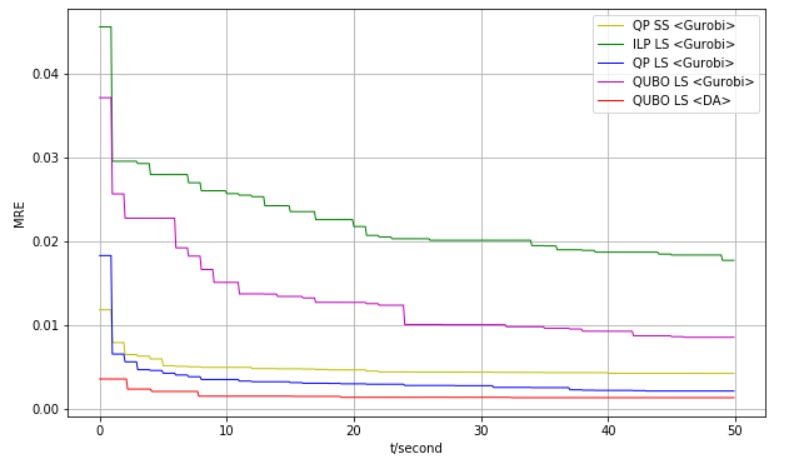
\includegraphics[width=\textwidth]{energy_50.png}  
	\caption{Mean Relative Energy (wrt best feasible solution) vs. Runtime (after 50 seconds).}%
	
	\label{fig:results1}%
\end{figure}

\begin{figure}[t]%
	
	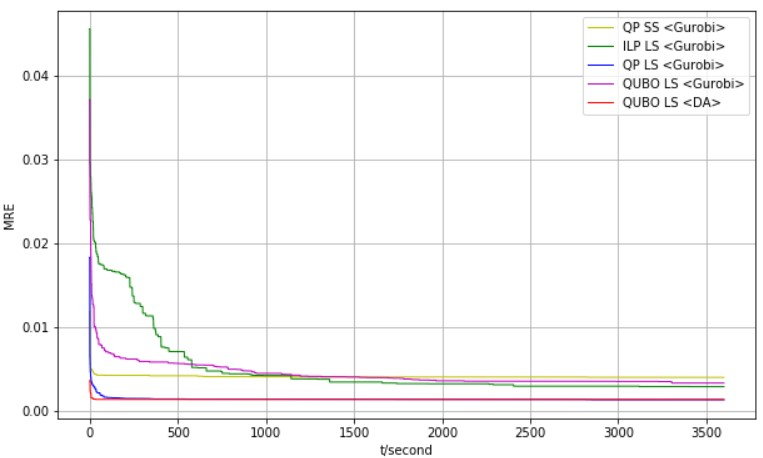
\includegraphics[width=\textwidth]{energy_3600.png}   \\%\\
	\caption{Mean Relative Energy (wrt best feasible solution) vs. Runtime (after 3600 seconds).}%
	
	\label{fig:results2}%
\end{figure}



\section{Discussion and Practical Implications}
\label{sec:discussion}

Our results show numerically that the quadratic programming models that we
introduced in Section~\ref{sec:QUBO4WFLO} (\qcls{} and \quls{}) are useful in two ways.
First, the two methods are powerful approaches to solving WFLO. Specifically, \qcls{} yields the best performance (after 3600 seconds) for most problem instances
and especially,
for the hard instances with 36 wind directions. In addition, the runtime performance of \qcls{} is second
only to the Digital Annealer.  Second, the QUBO model can be solved with recent specialized hardware, Fujitsu's DA, as demonstrated by the \qulsda{} approach. \qulsda{} yields the best results in 7 out of 12 
instances, shows competitive performance on the other instances, and outperforms all methods in terms of performance in short runtimes (a speed-up factor of 3 orders of magnitude when the DA runs for $1$ second).



The ability of \qulsda{} to quickly obtain competitive solutions on large WFLO instances 
is crucial when iteratively solving
multiple wind farm layout problems at design time. Moreover, it allows the flexibility to tune the various WFLO parameters (including turbine specs, number of turbines, and farm sizes) without incurring a steep computational cost that come
with (re-)solving the problem using exact methods. The quality loss due to the use of an approximate method 
that exploits advanced technology is negligible. This balance between
runtime and total energy, points at the potential contribution of the proposed quadratic framework for solving WFLO. 

Finally, though we have not emphasized it here, all the approaches presented, including those from the literature, have the advantage of being represented with a declarative mathematical model. Such a representation makes problem extensions significantly easier and allows formal analysis. While model-based  approaches are common in exact optimization such as mixed-integer programming, they are rare for heuristic techniques such as genetic algorithms and meta-heuristics. Many of the state-of-the-art implementations of heuristic techniques are specialized for the particular problem being solved. A change in the problem definition (e.g., the addition of a new constraint) can, therefore, require substantial software changes. Conversely, model-based techniques can be adapted to a revised problem definition via the declarative addition of the new constraint to the model. Further, amenability to formal analysis means that substantial insight can be gained from mathematical treatments of problem classes, leading, as can be seen in mixed integer programming \cite{Bixby07a}, to substantial improvements in problem solving performance.

%State-of-the-art solvers still make use of advanced data structures but they are specialized for the class of problems expressible in the mathematical formalism rather than the problem at hand. Additionally, the mathematical representation of the model allows formal results to be proved. Model-based approaches can therefore provide 

  
\section{Conclusion}
\label{sec:conclusion}

In this work, we presented a novel quadratic programming framework
for solving 
wind farm layout optimization. 
The framework is embodied in two models: constrained (\qcls) and unconstrained binary
 (\quls) quadratic programs. The former can be used to solve WFLO using advanced optimization software,
while the latter can be mounted onto specialized hardware that can quickly (approximately) solve WFLO. We used the constrained quadratic formulation to prove 
that the computational complexity of WFLO is $\mathcal{NP}$-hard. Nonetheless,
our numerical evaluation shows that when exact solvers like Gurobi~\cite{gurobi} are
coupled with our \qcls{} and \quls{} models they are able to solve small WFLO instances to optimality in less than 3600 seconds.
We also show that when an advanced hardware is used with the QUBO representation, large WFLO instances can be solved quickly with no significant degradation in the total energy compared to exact methods.
This runtime improvement and state-of-the-art performance in terms of the total energy of the resulting solutions makes our quadratic framework useful for designing new wind farms, while varying multiple input parameters. 


In future work, we aim at extending our quadratic models to include additional 
WFLO aspects, such as noise, non-flat terrain, and multiple objectives. 
Moreover, we wish to explore real-world wind farm design problems 
that may be larger and more complex than the 12 standard instances 
and solve them 
using our quadratic programming approaches. 



\appendix

\section{Speedup Results}
\label{app1}



\begin{table}[t!]
	\small
	\begin{tabular}{| c | c | c | c | c | c | }
		\toprule
		Wind Directions  & n  & m  & \qcls &  \ilpls & \qulsgrb  \\
		\toprule
		\multirow{6}{*}{WR1}  & \multirow{3}{*}{10}  & 20 & 1       & 1 & 1  \\
		& & 30   & N/A & N/A & 1     \\
		& & 40 & 1 & 1 & N/A                \\
		\cline{2-6}
		&\multirow{3}{*}{20}   & 20  & 1  & 1  & 259         \\
		&&30   & 3 & 2  & 9    \\
		&&40   & 32 & 22  & 602        \\
		\hline
		\multirow{6}{*}{WR36} &  \multirow{3}{*}{10}    & 20 & 1       & 1661 & 1  \\
		&& 30  & 3600 & 3600 & 3600                     \\
		&&40   & 1 & 3600 & 1          \\
		\cline{2-6}
		&  \multirow{3}{*}{20}   & 20   & 3600  & 538 & 944            \\
		&&30   & 22 & 3600 & 3304                     \\
		&&40   & 60 & 3600 & 1717 \\
		\bottomrule                   
	\end{tabular}
	
	\vspace{0.5em}
	\caption{Speedup factor per LS-based method for all instances w.r.t \qulsda{} at 1 second. The value 3600 implies a lower bound on the speedup factor.}\label{tab:results3}
\end{table}




\begin{table}[t!]
	\small
	\begin{tabular}{| c | c | c | c | c | c | }
		\toprule
		Wind Directions  & n  & m  & \qcls &  \ilpls & \qulsgrb  \\
		\toprule
		\multirow{6}{*}{WR1}  & \multirow{3}{*}{10}  & 20 & 0.1       & 0.1 & 0.1  \\
		& & 30   & N/A & N/A & 0.1     \\
		& & 40 & 0.1 & 0.1 & N/A                \\
		\cline{2-6}
		&\multirow{3}{*}{20}   & 20  & 1  & 1  & 25.9         \\
		&&30   & 0.3 & 0.2  & 0.9    \\
		&&40   & 6.1 & 2.2  & 360        \\
		\hline
		\multirow{6}{*}{WR36} &  \multirow{3}{*}{10}    & 20 & 0.1       & 360 & 0.2  \\
		&& 30  & 360 & 360 & 360                     \\
		&&40   & 0.1 & 360 & 0.1          \\
		\cline{2-6}
		&  \multirow{3}{*}{20}   & 20   & 360  & 360 & 360            \\
		&&30   &  360  & 360 & 360                    \\
		&&40   &  8  & 360 & 360 \\
		
		\bottomrule                   
	\end{tabular}
	
	\vspace{0.5em}
	\caption{Speedup factor per LS-based method for all instances w.r.t \qulsda{} at 10 second. The value 360 implies a lower bound on the speedup factor.}\label{tab:results4}
\end{table}
Table~\ref{tab:results3} presents the speedup results across all problem instances
for every LS-based method (computed using the SS energy term). The speedup is calculated according to Eq.~(\ref{eq:speedup}). Table~\ref{tab:results4} shows similar results for the speedup factor
compared to DA at 10 seconds. The average lower bound on the speedup at $1$ seconds
is 665,	1511, and 949 for \qclsgrb, \qulsgrb, and \ilplsgrb, respectively. For the $10$ second
results, the average
speedup factor is at least 99, 196, and	166 for the respective methods.
For instances where the speedup factor in Table~\ref{tab:results4} is 10 times less than in Table~\ref{tab:results3},
the DA found the 10-second solution after 1 second.

Note that the ``N/A'' values in the table arise from our use of two different energy functions, $E_{SS}$ and $E_{LS}$. For some problem instances, an exact solver for \qcls{} finds and proves an optimal solution for the $E_{LS}$ objective but, when that solution is evaluated using the $E_{SS}$ energy function, it has a lower energy than the solution found by the DA. This phenomenon is correct because the mapping from $E_{LS}$ to $E_{SS}$ does not necessarily preserve the ordering of solution quality. We do not include these instances in our speedup computations.  



\bibliographystyle{elsarticle-num-names}
%\bibliographystyle{plainnat}
\bibliography{Biblio}



\end{document}



%
%\begin{table}[t]
%	
%
%	\label{tab:results1}
%	\vspace{-0.5em}
%	\scriptsize
%	\centering
%	\begin{tabular}{ c @{\hspace{1em}} c @{\hspace{1em}} c @{\hspace{1em}} c}
%		\toprule
%		Paper & Exact Optimization & Discrete Grid & Flat Terrain  \\
%		\midrule
%		\citet{Zhang2014,turner2014new} & + & + & +  \\
%		\citet{kuo2016wind} & + & + & -  \\
%		 \citet{} & + & - & + \\
%		
%		\bottomrule
%	\end{tabular}
%	\vspace{-1em}
%	\caption{Literature review of Wind Farm Optimization Layout solutions.}
%		
%\end{table}


